% Generated by generate_human_review_tables.py.
\begin{figure}[htbp]
\centering
\caption{Adequação entre entregas e disponibilidade de respostas adequadas}
\label{fig:adequacao_disponibilidade}
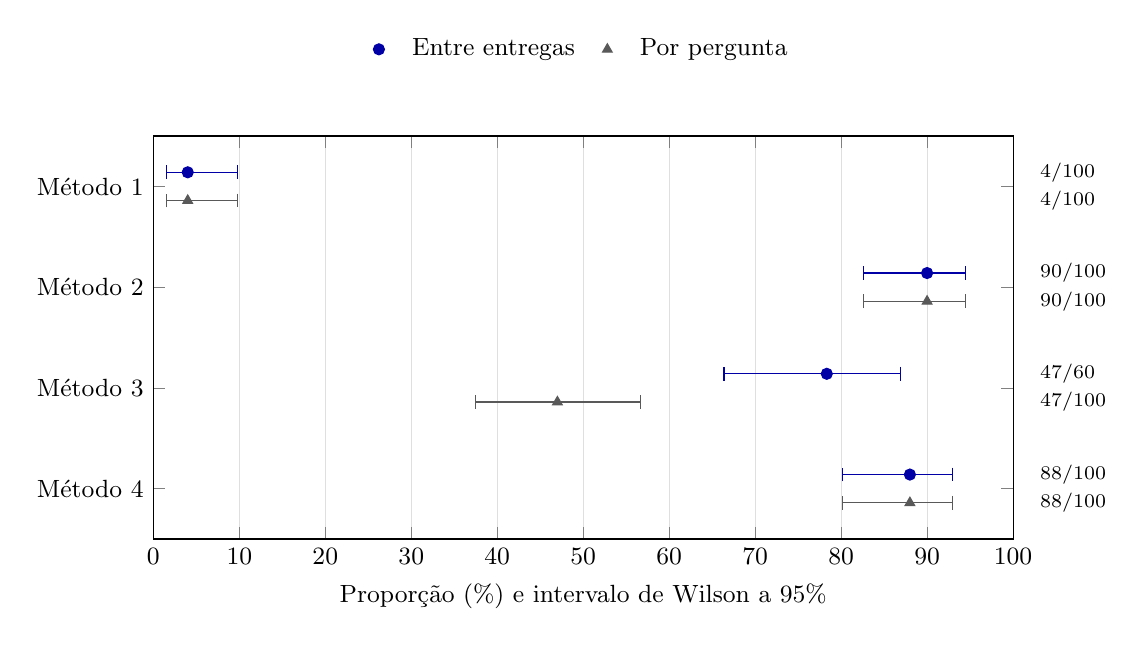
\begin{tikzpicture}
\begin{axis}[
    width=12.5cm,height=6.7cm,xmin=0,xmax=100,ymin=0.5,ymax=4.5,y dir=reverse,
    xlabel={Proporção (\%) e intervalo de Wilson a 95\%},
    ytick={1,2,3,4},yticklabels={Método 1,Método 2,Método 3,Método 4},
    xmajorgrids=true,grid style={gray!25},clip=false,
    tick label style={font=\small},label style={font=\small},
    legend style={at={(0.5,1.16)},anchor=south,draw=none,font=\small,column sep=8pt},legend columns=2]
\addplot+[only marks,mark=*,color=blue!65!black,mark options={draw=blue!65!black,fill=blue!65!black},error bars/.cd,x dir=both,x explicit,error mark options={rotate=90,mark size=2.5pt}] coordinates {(4,0.860) += (5.83707144,0) -= (2.4336696,0) (90,1.860) += (4.47708629,0) -= (7.43656615,0) (78.3333333,2.860) += (8.54362262,0) -= (11.9533609,0) (88,3.860) += (5.00059356,0) -= (7.81209943,0)};
\addplot+[only marks,mark=triangle*,color=black!65,mark options={draw=black!65,fill=black!65},error bars/.cd,x dir=both,x explicit,error mark options={rotate=90,mark size=2.5pt}] coordinates {(4,1.140) += (5.83707144,0) -= (2.4336696,0) (90,2.140) += (4.47708629,0) -= (7.43656615,0) (47,3.140) += (9.71114303,0) -= (9.48918204,0) (88,4.140) += (5.00059356,0) -= (7.81209943,0)};
\node[anchor=west,font=\scriptsize] at (axis cs:102,0.860) {4/100};
\node[anchor=west,font=\scriptsize] at (axis cs:102,1.140) {4/100};
\node[anchor=west,font=\scriptsize] at (axis cs:102,1.860) {90/100};
\node[anchor=west,font=\scriptsize] at (axis cs:102,2.140) {90/100};
\node[anchor=west,font=\scriptsize] at (axis cs:102,2.860) {47/60};
\node[anchor=west,font=\scriptsize] at (axis cs:102,3.140) {47/100};
\node[anchor=west,font=\scriptsize] at (axis cs:102,3.860) {88/100};
\node[anchor=west,font=\scriptsize] at (axis cs:102,4.140) {88/100};
\legend{Entre entregas,Por pergunta}
\end{axis}
\end{tikzpicture}
\fonte{Julgamentos globais realizados pelo autor. À direita constam numerador e denominador de cada medida. Os intervalos descrevem proporções individuais e não testam diferenças entre métodos.}
\end{figure}
